% Chapter Template
\chapter{Results} % Main chapter title

\label{Results} % Change X to a consecutive number; for referencing this chapter elsewhere, use \ref{ChapterX}

This chapter presents findings from the experiments conducted to evaluate Sarosh’s Perceptron Networks (SPNs) against traditional Multi-Layer Perceptrons (MLPs), addressing the research questions outlined in Chapter \ref{Introduction}. The results are organized into three sections corresponding to the domains evaluated: Images, Tabular Data, and Text Data. For each domain, results from all model architectures detailed in Chapter \ref{Experiments} are presented, compared, and analyzed.

Throughout this chapter, shorter representations for model names and evaluations have been adopted for clarity:

\begin{table}[h!]
    \centering
    \begin{tabular}{ll}
    \textbf{Full name} & \textbf{Representation used} \\
    \hline
    Models: & \\
    \hspace{1em} Baseline MLP & base\_mlp \\
    \hspace{1em} Free Weights SPN & fw\_spn \\
    \hspace{1em} Minimal SPN & min\_spn \\
    \hspace{1em} Minimal MLP & min\_mlp \\
    \hspace{1em} Maximal SPN & max\_spn \\
    \hspace{1em} Pruned Maximal SPN & pruned\_spn \\
    Evaluation Metrics: & \\
    \hspace{1em} Parameter Count & param\_count \\
    \hspace{1em} Best Test Accuracy & best\_acc \\
    \hspace{1em} Time to Best Accuracy & time\_best \\
    \hspace{1em} Training Efficiency & train\_eff \\
    \hspace{1em} Area Under Curve Efficiency & auc\_eff \\
    \hspace{1em} Throughput Efficiency & thru\_eff \\
    \end{tabular}
\end{table}

%----------------------------------------------------------------------------------------
%	SECTION 1
%----------------------------------------------------------------------------------------

\section{Image Domain Results}

Both image datasets were flattened and normalized before model training.

\subsection{MNIST Dataset}

\begin{tabular}{@{}ll@{}}
\textbf{Variant} & Simple \\
\textbf{Input Features} & 784 \\
\textbf{Output Classes} & 10 \\
\textbf{Batch Size} & 75 \\
\textbf{Training Epochs} & 50 \\
\textbf{Training Samples} & 60,000 \\
\textbf{Test Samples} & 10,000 \\
\textbf{Base MLP Dimensions} & $[12,\, 12,\, 10]$ \\
\textbf{Total Neurons} & 34 \\
\end{tabular}

Hellobib \cite{pwc_mnist_leaderboard}

\begin{figure}[H]
    \centering
    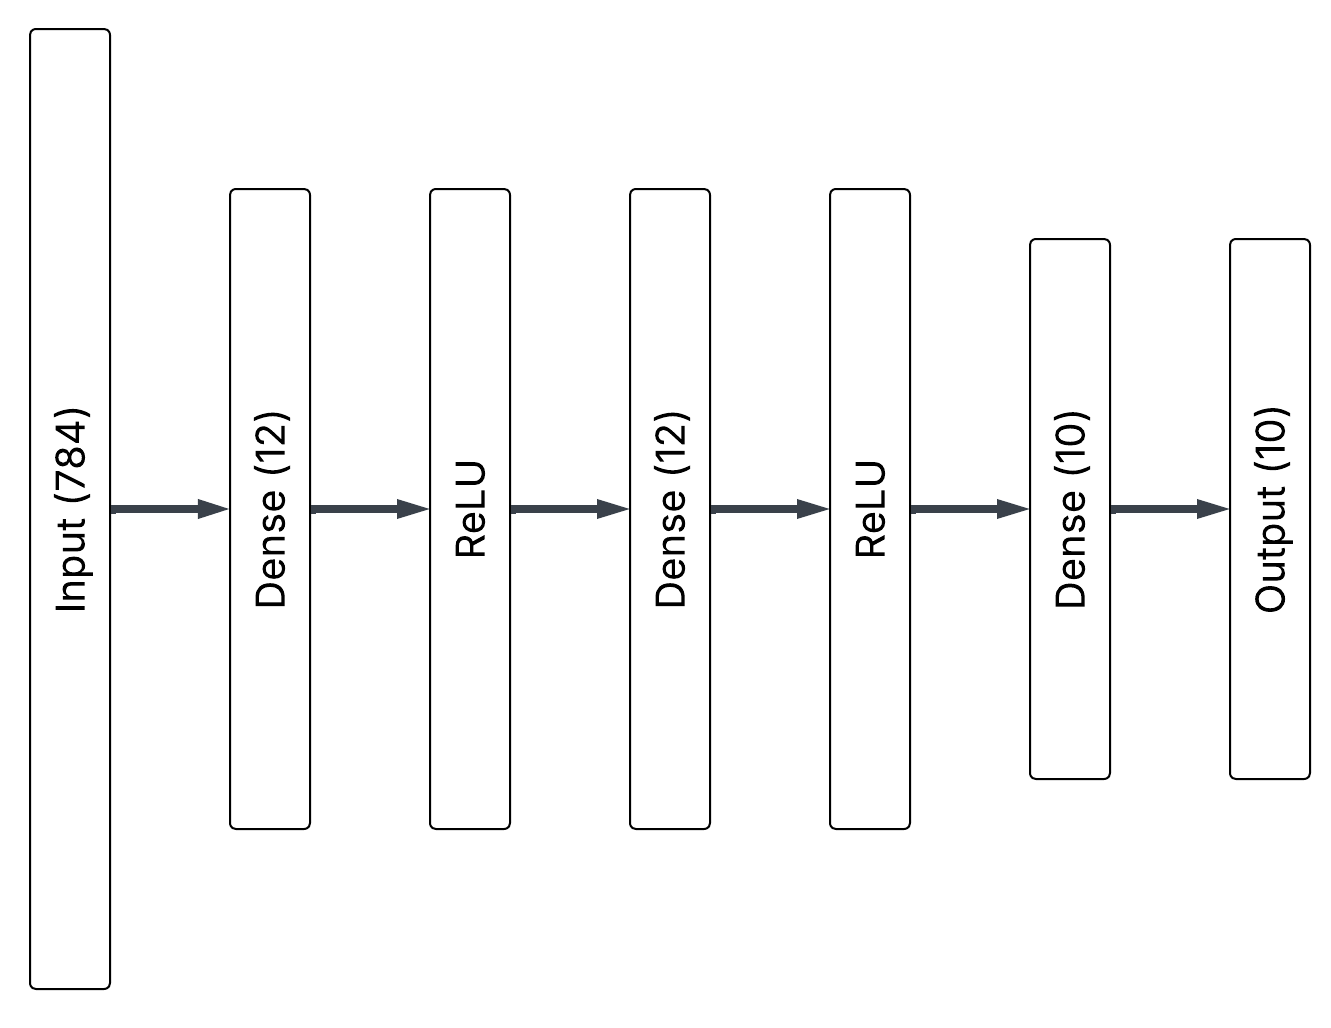
\includegraphics[width=0.6\textwidth]{Figures/Results/MNIST/MNIST_base_mlp_architecture.png} 
    \captionsetup{justification=centering}  % Ensure the caption is centered
    \caption{base\_mlp architecture for MNIST}
    \label{fig:mnistMlpBaseArch}
\end{figure}

The training and testing curves in Figures \ref{fig:mnistTrainCurve} and \ref{fig:mnistTestCurve} clearly demonstrate that the min\_mlp and base\_mlp models underperform relative to all SPN models. Table \ref{tab:mnistResults} offers a detailed comparison of all six models across the efficiency metrics.

\begin{figure}[H]
    \centering
    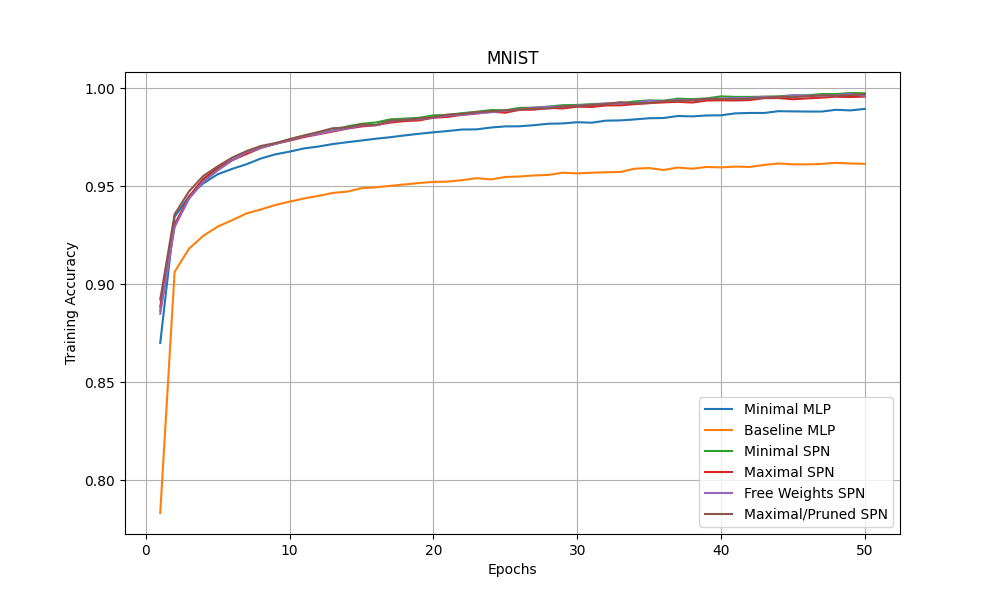
\includegraphics[width=\linewidth]{Figures/Results/MNIST/training_accuracy_plot.png} % first figure itself
    \captionsetup{width=\linewidth}
    \caption{train\_acc vs epochs curve for MNIST}
    \label{fig:mnistTrainCurve}
\end{figure}

\begin{figure}[H]
    \centering
    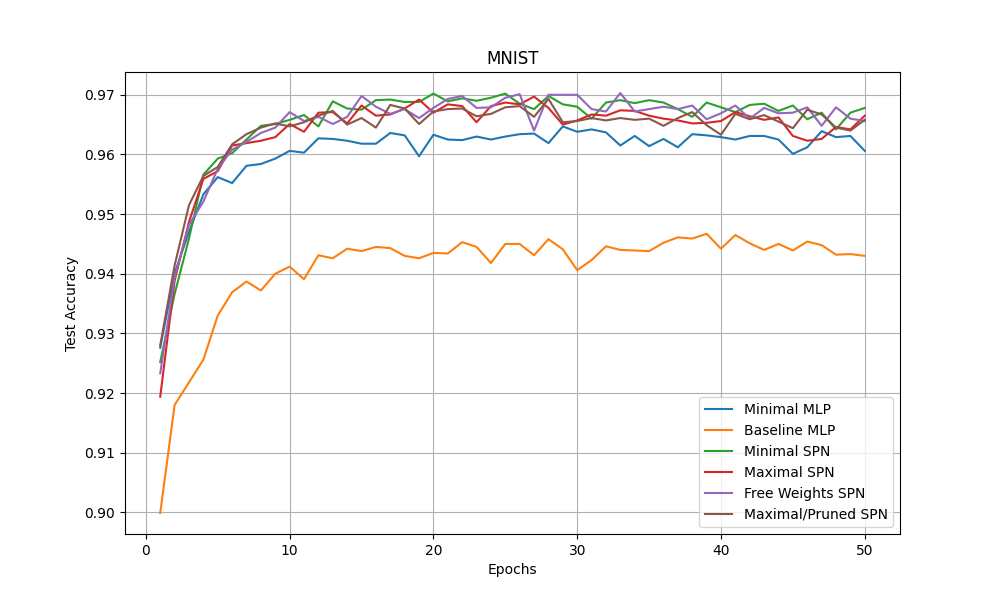
\includegraphics[width=\linewidth]{Figures/Results/MNIST/test_accuracy_plot.png} % second figure itself
    \captionsetup{width=\linewidth}
    \caption{test\_acc vs epochs curve for MNIST}
    \label{fig:mnistTestCurve}
\end{figure}

\begin{table}[h!]
    \centering
    \begin{tabular}{|l|l|l|l|l|l|l|}
    \hline
    \textbf{Model} & \textbf{param\_count} & \textbf{best\_acc} & \textbf{time\_best} & \textbf{train\_eff} & \textbf{auc\_eff} & \textbf{thru\_eff} \\
    \hline
    base\_mlp & 9,706 & \cellcolor{red!25}94.67\% & 45.34s & 0.021 & \cellcolor{red!25}46.131 & 0.816 \\
    fw\_spn & 27,074  & \cellcolor{green!25}97.03\% & 53.09s  & 0.018 & 47.297 & 0.607 \\
    min\_spn & 26,930 & 97.02\% & \cellcolor{green!25}18.23  & \cellcolor{green!25}0.053 & \cellcolor{green!25}47.318 & 1.043 \\
    min\_mlp & 19,090 & 96.47\% & 24.85s & 0.039 & 47.074 & \cellcolor{green!25}1.127 \\
    max\_spn & 27,251  & 96.97\% & \cellcolor{red!25}399.87s & \cellcolor{red!25}0.002 & 47.246 & \cellcolor{red!25}0.064 \\
    pruned\_spn & 27,025 & 96.93\% & 44.99s & 0.022 & 47.256 & 0.595 \\
    \hline
    \end{tabular}
    \caption{Cross Model Comparison on the MNIST dataset}
    \label{tab:mnistResults}
\end{table}

\begin{enumerate}
\item \textbf{Baseline MLP vs. Free Weights SPN}: The fw\_spn model achieved the highest test accuracy, clearly outperforming the base\_mlp, which had the lowest accuracy out of all the models. The notable increase in parameter count of the fw\_spn, while retaining the same layer layout as the base\_mlp, correlates positively with its improved accuracy, providing strong evidence that enhanced internal connectivity boosts model performance. Although fw\_spn had slightly lower training and throughput efficiencies than the base\_mlp, this trade-off was justified by the considerable gain in accuracy.
\item \textbf{Minimal MLP vs. Minimal SPN}: Both min\_spn and min\_mlp achieved better accuracy compared to base\_mlp but slightly lower than fw\_spn. This suggests that having a higher param\_count might be more advantageous in this dataset than having more layers. Min\_spn consistently outperformed min\_mlp across all metrics except throughput efficiency, where both models were fairly close to one another. This further emphasizes the benefit of increased neural connectivity on model performance.
\item \textbf{Maximal SPN}: Max\_spn model had the third-highest accuracy but required significantly longer training times compared to the other models. This suggests a performance ceiling for the MNIST dataset, where additional internal connections yield diminishing returns.
\item \textbf{Pruned SPN}:
\begin{center}  % Centers the table
\begin{tabular}{|l|l|}
\hline
\textbf{Metric} & \textbf{Value} \\
\hline
Layers Before Pruning & 34 \\
Layers After Pruning & 3 \\
Mean Epoch Time Before Pruning & 15.89s \\
Mean Epoch Time After Pruning & 1.59s \\
Pruning Time & 631.68s \\
Pruning Effectiveness & 9.99 \\
\hline
\end{tabular}
\end{center}

The pruned\_spn model achieved accuracy similar to max\_spn while dramatically improving computational efficiency. Although the pruning process itself was time-consuming, taking longer than it took max\_spn to reach its peak accuracy (making it practically unusable), it still made the max\_spn model nearly 10x faster in average training time, validating the efficacy of pruning for optimizing maximal SPNs. Additionally, this pruning confirmed that a three-layer architecture is sufficient for optimal performance on this dataset. 

However, since max\_spn did not outperform any of the other models, it suggests that there was limited additional learning to be done, making pruning easier on this particular dataset.
\end{enumerate}

Overall, SPNs convincingly outperformed their MLP counterparts on the MNIST dataset. Maximal and pruned SPNs confirmed the existence of an upper performance bound, highlighting the effectiveness of strategic pruning to balance accuracy and efficiency.

\subsection{CIFAR 10 Dataset}

\begin{tabular}{@{}ll@{}}
\textbf{Variant} & Complex \\
\textbf{Input Features} & 3072 \\
\textbf{Output Classes} & 10 \\
\textbf{Batch Size} & 128 \\
\textbf{Training Epochs} & 30 \\
\textbf{Training Samples} & 50,000 \\
\textbf{Test Samples} & 10,000 \\
\textbf{Base MLP Dimensions} & $[256,\, 128,\, 64,\, 32,\, 10]$ \\
\textbf{Total Neurons} & 490 \\
\end{tabular}

\begin{figure}[H]
    \centering
    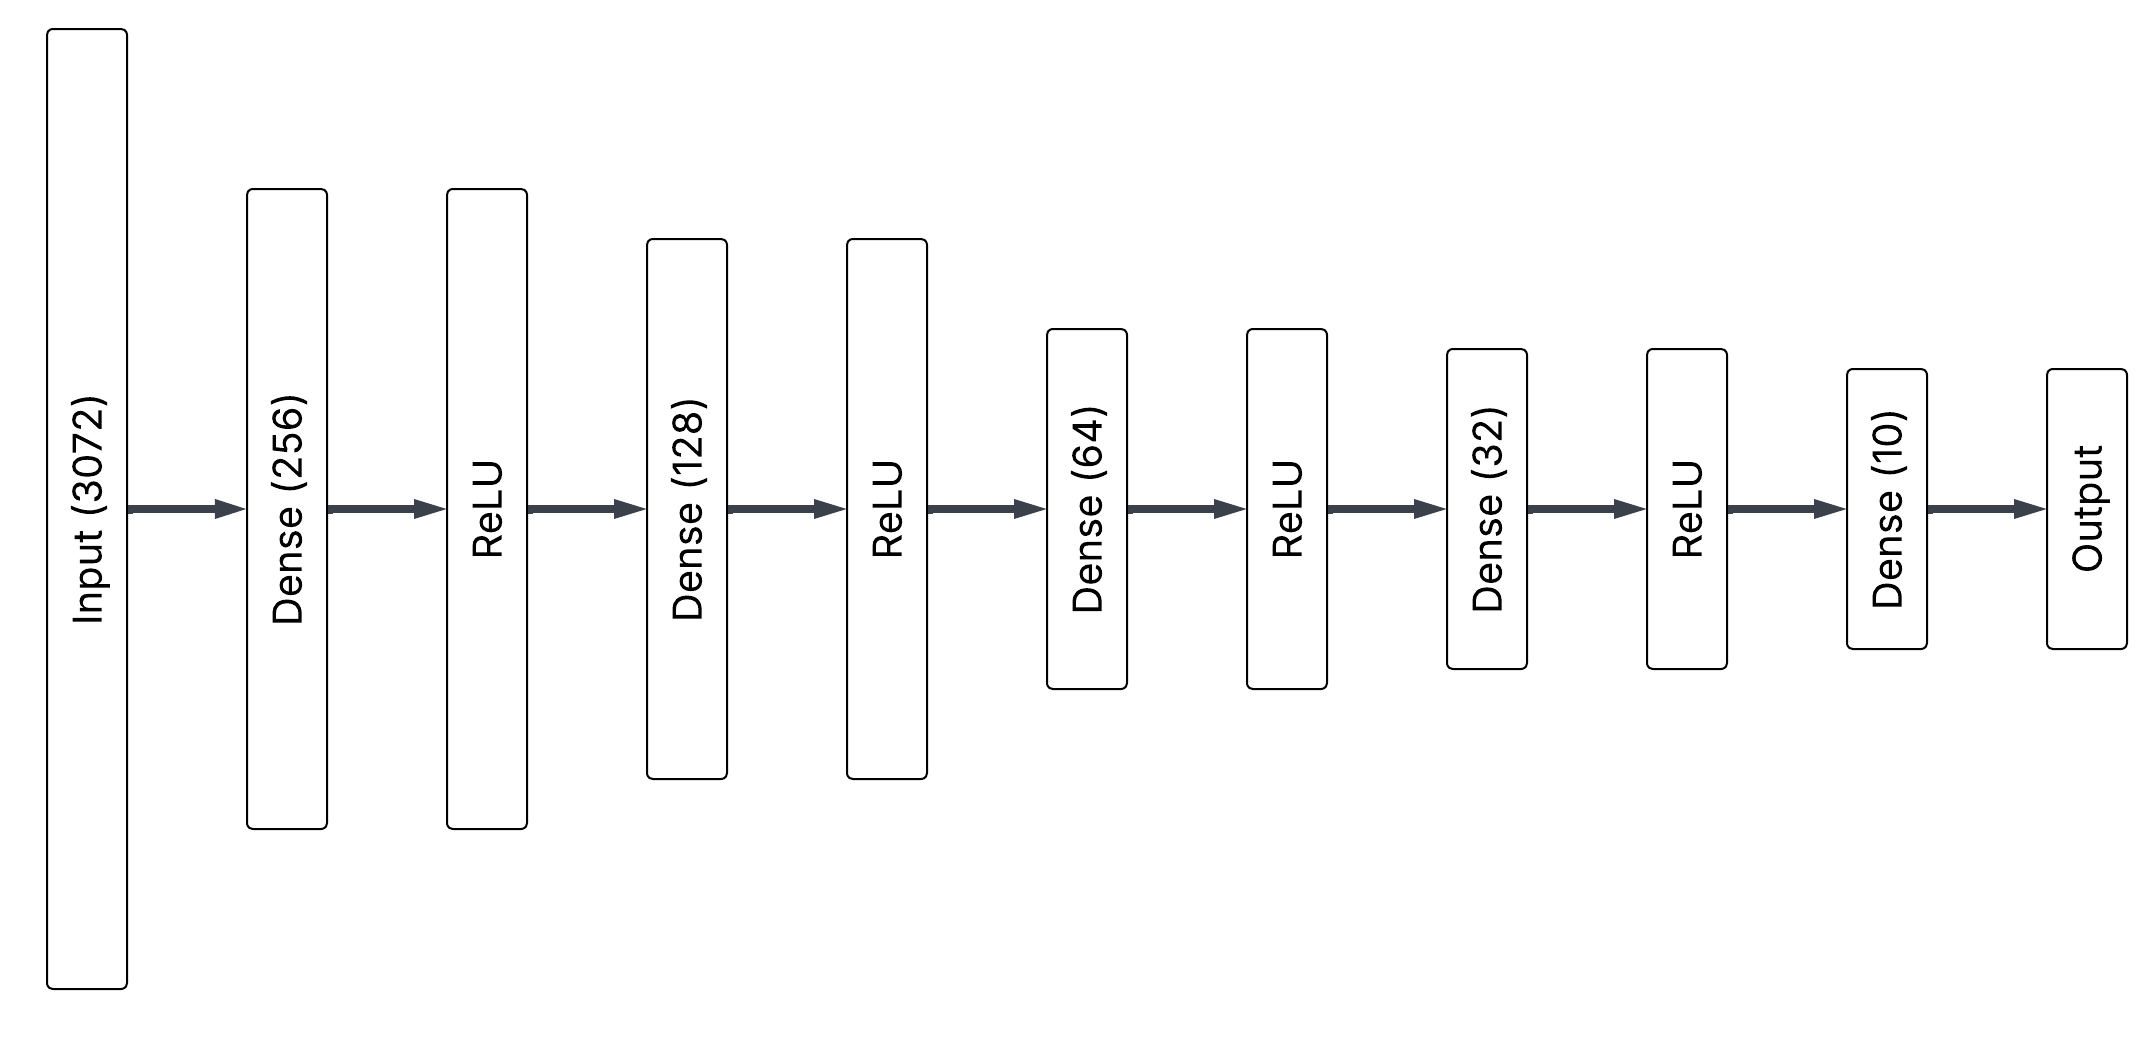
\includegraphics[width=1.0\textwidth]{Figures/Results/CIFAR_10/CIFAR_base_mlp_architecture.png} 
    \captionsetup{justification=centering}  % Ensure the caption is centered
    \caption{base\_mlp architecture for CIFAR 10}
    \label{fig:cifarMlpBaseArch}
\end{figure}

\begin{figure}[H]
    \centering
    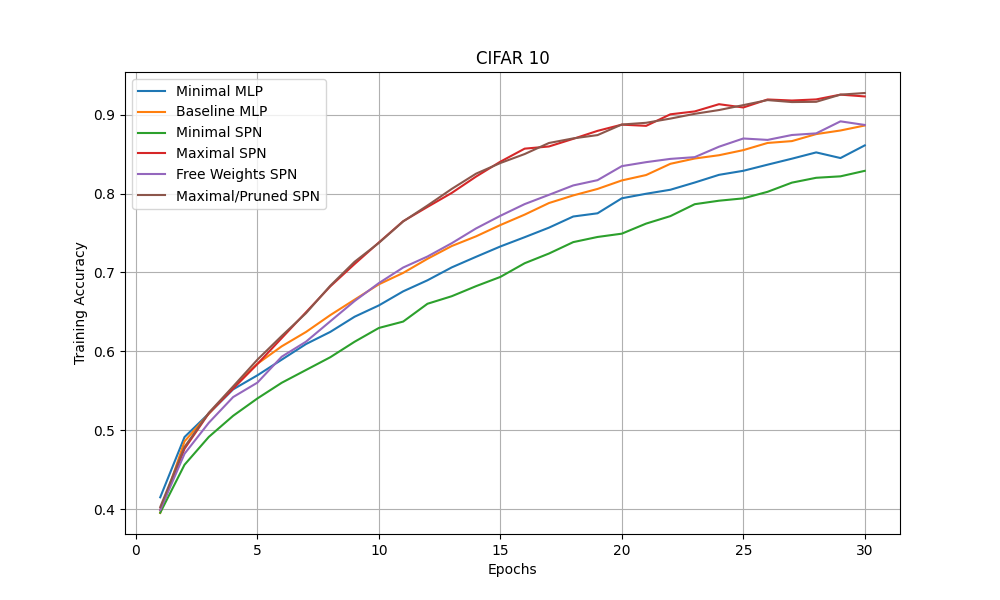
\includegraphics[width=\linewidth]{Figures/Results/CIFAR_10/training_accuracy_plot.png} % first figure itself
    \captionsetup{width=\linewidth}
    \caption{train\_acc vs epochs curve for CIFAR 10}
    \label{fig:cifarTrainCurve}
\end{figure}

\begin{figure}[H]
    \centering
    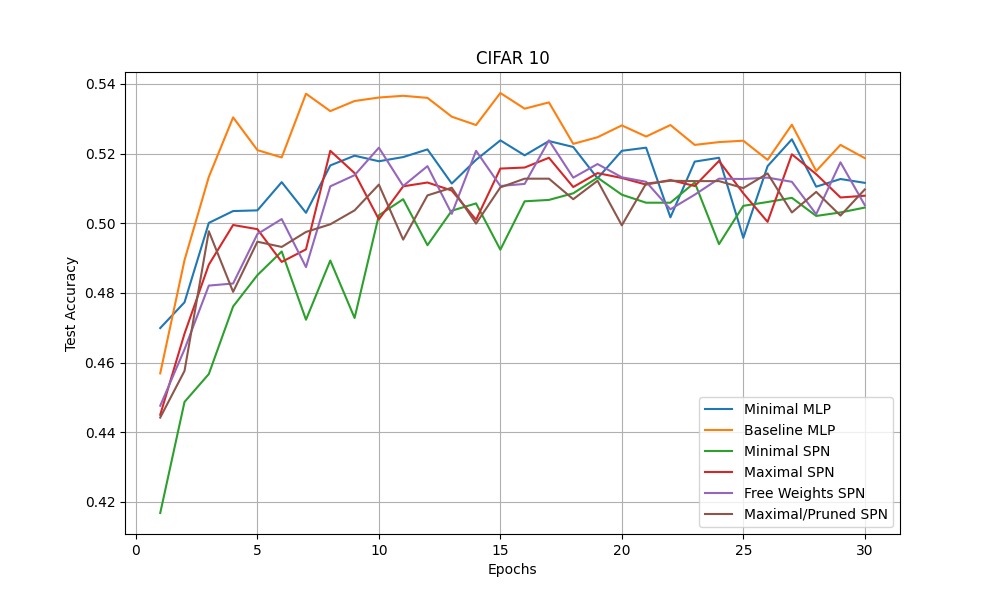
\includegraphics[width=\linewidth]{Figures/Results/CIFAR_10/test_accuracy_plot.png} % second figure itself
    \captionsetup{width=\linewidth}
    \caption{test\_acc vs epochs curve for CIFAR 10}
    \label{fig:cifarTestCurve}
\end{figure}

\begin{table}[h!]
    \centering
    \begin{tabular}{|l|l|l|l|l|l|l|}
    \hline
    \textbf{Model} & \textbf{param\_count} & \textbf{best\_acc} & \textbf{time\_best} & \textbf{train\_eff} & \textbf{auc\_eff} & \textbf{thru\_eff} \\
    \hline
    base\_mlp & 830,250 & \cellcolor{green!25}53.74\% & 14.12s & 0.038 & \cellcolor{green!25}15.220 & 0.585 \\
    fw\_spn & 1,582,250 & 52.38\% & 19.57s & 0.027 & 14.671 & 0.449 \\
    min\_spn & 1,510,570 & \cellcolor{red!25}51.31\% & \cellcolor{green!25}10.60s & \cellcolor{green!25}0.048 & \cellcolor{red!25}14.342 & 0.925 \\
    min\_mlp & 1,479,850 & 52.41\% & 12.83s & 0.041 & 14.856 & \cellcolor{green!25}1.100 \\
    max\_spn & 1,625,575 & 52.08\% & \cellcolor{red!25}472.26s & \cellcolor{red!25}0.001 & 14.672 & \cellcolor{red!25}0.009 \\
    pruned\_spn & 1,623,931 & 51.43\% & 453.08s & \cellcolor{red!25}0.001 & 14.567 & 0.029 \\
    \hline
    \end{tabular}
    \caption{Cross Model Comparison on the CIFAR 10 Dataset}
    \label{tab:cifarResults}
\end{table}

\begin{enumerate}
\item \textbf{Baseline MLP vs. Free Weights SPN}: The fw\_spn model achieved the highest test accuracy, clearly outperforming the base\_mlp, which had the lowest accuracy out of all the models. The notable increase in parameter count of the fw\_spn, while retaining the same layer layout as the base\_mlp, correlates positively with its improved accuracy, providing strong evidence that enhanced internal connectivity boosts model performance. Although fw\_spn had slightly lower training and throughput efficiencies than the base\_mlp, this trade-off was justified by the considerable gain in accuracy.
\item \textbf{Minimal MLP vs. Minimal SPN}: Both min\_spn and min\_mlp achieved better accuracy compared to base\_mlp but slightly lower than fw\_spn. This suggests that having a higher param\_count might be more advantageous in this dataset than having more layers. Min\_spn consistently outperformed min\_mlp across all metrics except throughput efficiency, where both models were fairly close to one another. This further emphasizes the benefit of increased neural connectivity on model performance.
\item \textbf{Maximal SPN}: Max\_spn model had the third-highest accuracy but required significantly longer training times compared to the other models. This suggests a performance ceiling for the MNIST dataset, where additional internal connections yield diminishing returns.
\item \textbf{Pruned SPN}:
\begin{center}  % Centers the table
\begin{tabular}{|l|l|}
\hline
\textbf{Metric} & \textbf{Value} \\
\hline
Layers Before Pruning & 34 \\
Layers After Pruning & 86 \\
Mean Epoch Time Before Pruning & 62.06s \\
Mean Epoch Time After Pruning & 17.85s \\
Pruning Time & 1520.61s \\
Pruning Effectiveness & 3.48 \\
\hline
\end{tabular}
\end{center}
The pruned\_spn model achieved accuracy similar to max\_spn while dramatically improving computational efficiency. Although the pruning process itself was time-consuming, taking longer than it took max\_spn to reach its peak accuracy (making it practically unusable), it still made the max\_spn model nearly 10x faster in average training time, validating the efficacy of pruning for optimizing maximal SPNs. Additionally, this pruning confirmed that a three-layer architecture is sufficient for optimal performance on this dataset. 

However, since max\_spn did not outperform any of the other models, it suggests that there was limited additional learning to be done, making pruning easier on this particular dataset.
\end{enumerate}

Overall, SPNs convincingly outperformed their MLP counterparts on the MNIST dataset. Maximal and pruned SPNs confirmed the existence of an upper performance bound, highlighting the effectiveness of strategic pruning to balance accuracy and efficiency.


\section{Tabular Domain Results}

\subsection{Titanic Dataset}

\begin{tabular}{@{}ll@{}}
\textbf{Variant} & Simple \\
\textbf{Input Features} & 7 \\
\textbf{Output Classes} & 2 \\
\textbf{Batch Size} & 32 \\
\textbf{Training Epochs} & 50 \\
\textbf{Training Samples} & 712 \\
\textbf{Test Samples} & 179 \\
\textbf{Base MLP Dimensions} & $[16,\, 8,\, 4,\, 2]$ \\
\textbf{Total Neurons} & 30 \\
\end{tabular}

\begin{figure}[H]
    \centering
    \includegraphics[height=0.28\textheight,width=0.7\textwidth]{Figures/Results/Titanic/titanic_base_mlp_architecture.png} 
    \captionsetup{justification=centering}  % Ensure the caption is centered
    \caption{base\_mlp architecture for Titanic}
    \label{fig:titanicMlpBaseArch}
\end{figure}

\begin{table}[h!]
    \centering
    \begin{tabular}{|l|l|l|l|l|l|l|}
    \hline
    \textbf{Model} & \textbf{param\_count} & \textbf{best\_acc} & \textbf{time\_best} & \textbf{train\_eff} & \textbf{auc\_eff} & \textbf{thru\_eff} \\
    \hline
    base\_mlp & 310 & \cellcolor{red!25}82.68\% & 0.86s & 0.960 & \cellcolor{red!25}39.369 & 22.032 \\
    fw\_spn & 520 & \cellcolor{green!25}83.24\% & 0.33s & 2.560 & 39.735 & 18.331 \\
    min\_spn & 296 & \cellcolor{red!25}82.68\% & \cellcolor{green!25}0.02s & \cellcolor{green!25}34.747 & \cellcolor{green!25}39.941 & 33.714 \\
    min\_mlp & 282 & \cellcolor{red!25}82.68\% & 0.09s & 9.020 & 39.802 & \cellcolor{green!25}36.282 \\
    max\_spn & 675 & \cellcolor{red!25}82.68\% & 1.72s & 0.482 & 39.430 & \cellcolor{red!25}2.376 \\
    pruned\_spn & 655 & \cellcolor{green!25}83.24\% & \cellcolor{red!25}8.05s & \cellcolor{red!25}0.103 & 39.503 & 4.746 \\
    \hline
    \end{tabular}
    \caption{Titanic Dataset results}
    \label{tab:titanicResults}
\end{table}

\begin{enumerate}
\item \textbf{Baseline MLP vs. Free Weights SPN}: The fw\_spn model achieved the highest test accuracy, clearly outperforming the base\_mlp, which had the lowest accuracy out of all the models. The notable increase in parameter count of the fw\_spn, while retaining the same layer layout as the base\_mlp, correlates positively with its improved accuracy, providing strong evidence that enhanced internal connectivity boosts model performance. Although fw\_spn had slightly lower training and throughput efficiencies than the base\_mlp, this trade-off was justified by the considerable gain in accuracy.
\item \textbf{Minimal MLP vs. Minimal SPN}: Both min\_spn and min\_mlp achieved better accuracy compared to base\_mlp but slightly lower than fw\_spn. This suggests that having a higher param\_count might be more advantageous in this dataset than having more layers. Min\_spn consistently outperformed min\_mlp across all metrics except throughput efficiency, where both models were fairly close to one another. This further emphasizes the benefit of increased neural connectivity on model performance.
\item \textbf{Maximal SPN}: Max\_spn model had the third-highest accuracy but required significantly longer training times compared to the other models. This suggests a performance ceiling for the MNIST dataset, where additional internal connections yield diminishing returns.
\item \textbf{Pruned SPN}:
\begin{center}  % Centers the table
\begin{tabular}{|l|l|}
\hline
\textbf{Metric} & \textbf{Value} \\
\hline
Layers Before Pruning & 30 \\
Layers After Pruning & 15 \\
Mean Epoch Time Before Pruning & 0.32s \\
Mean Epoch Time After Pruning & 0.18s \\
Pruning Time & 1.65s \\
Pruning Effectiveness & 1.78 \\
\hline
\end{tabular}
\end{center}
The pruned\_spn model achieved accuracy similar to max\_spn while dramatically improving computational efficiency. Although the pruning process itself was time-consuming, taking longer than it took max\_spn to reach its peak accuracy (making it practically unusable), it still made the max\_spn model nearly 10x faster in average training time, validating the efficacy of pruning for optimizing maximal SPNs. Additionally, this pruning confirmed that a three-layer architecture is sufficient for optimal performance on this dataset. 

However, since max\_spn did not outperform any of the other models, it suggests that there was limited additional learning to be done, making pruning easier on this particular dataset.
\end{enumerate}

\begin{figure}[H]
    \centering
    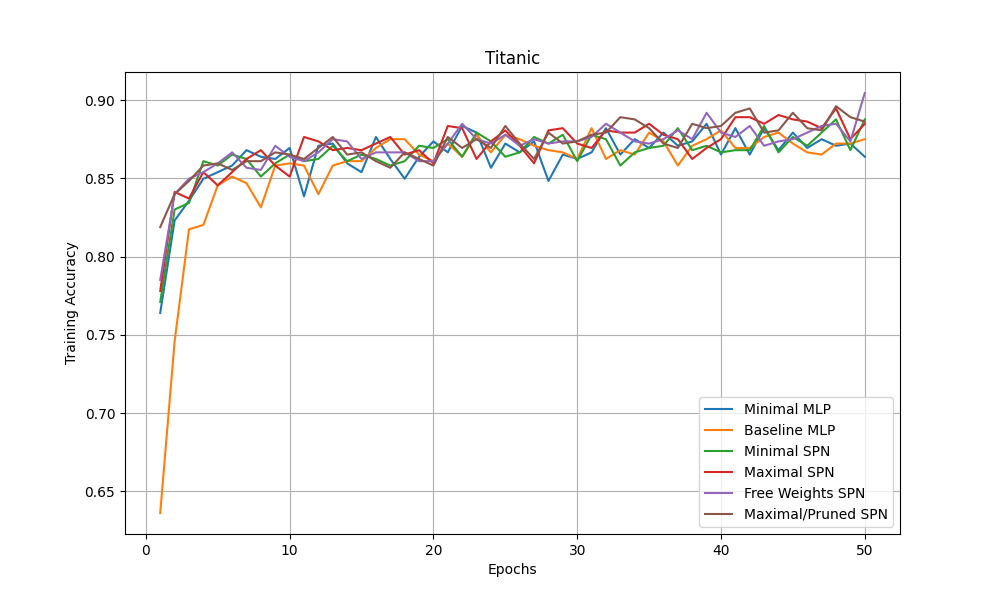
\includegraphics[width=\linewidth]{Figures/Results/Titanic/training_accuracy_plot.png} % first figure itself
    \captionsetup{width=\linewidth}
    \caption{train\_acc vs epochs curve for Titanic}
    \label{fig:titanicTrainCurve}
\end{figure}

\begin{figure}[H]
    \centering
    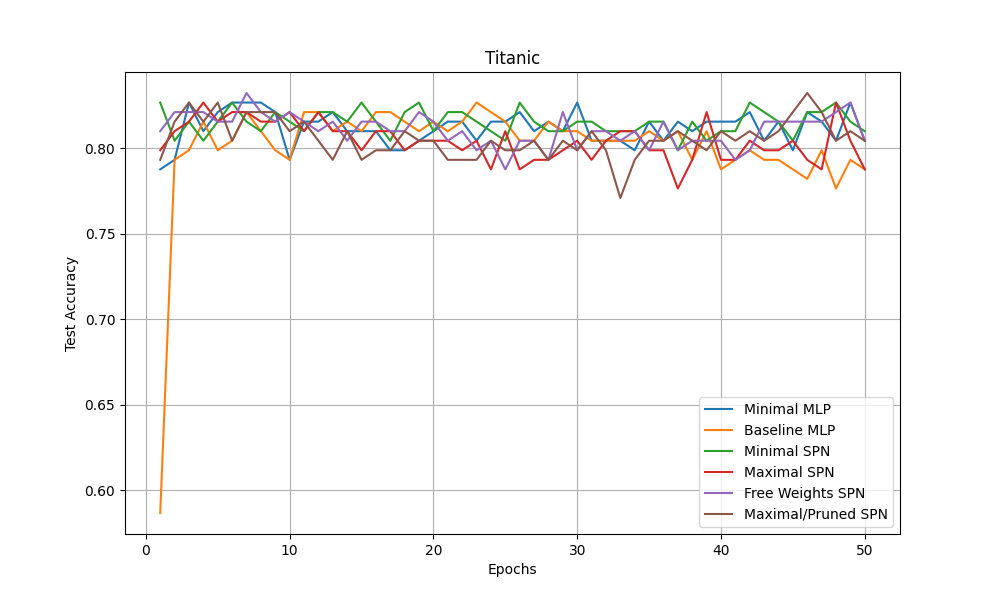
\includegraphics[width=\linewidth]{Figures/Results/Titanic/test_accuracy_plot.png} % second figure itself
    \captionsetup{width=\linewidth}
    \caption{test\_acc vs epochs curve for Titanic}
    \label{fig:titanicTestCurve}
\end{figure}

Overall, SPNs convincingly outperformed their MLP counterparts on the MNIST dataset. Maximal and pruned SPNs confirmed the existence of an upper performance bound, highlighting the effectiveness of strategic pruning to balance accuracy and efficiency.

\subsection{Covertype Dataset}

\begin{tabular}{@{}ll@{}}
\textbf{Variant} & Complex \\
\textbf{Input Features} & 54 \\
\textbf{Output Classes} & 7 \\
\textbf{Batch Size} & 256 \\
\textbf{Training Epochs} & 150 \\
\textbf{Training Samples} & 88,314 \\
\textbf{Test Samples} & 22,079 \\
\textbf{Base MLP Dimensions} & $[128,\, 64,\, 7]$ \\
\textbf{Total Neurons} & 199 \\
\end{tabular}

\begin{figure}[H]
    \centering
    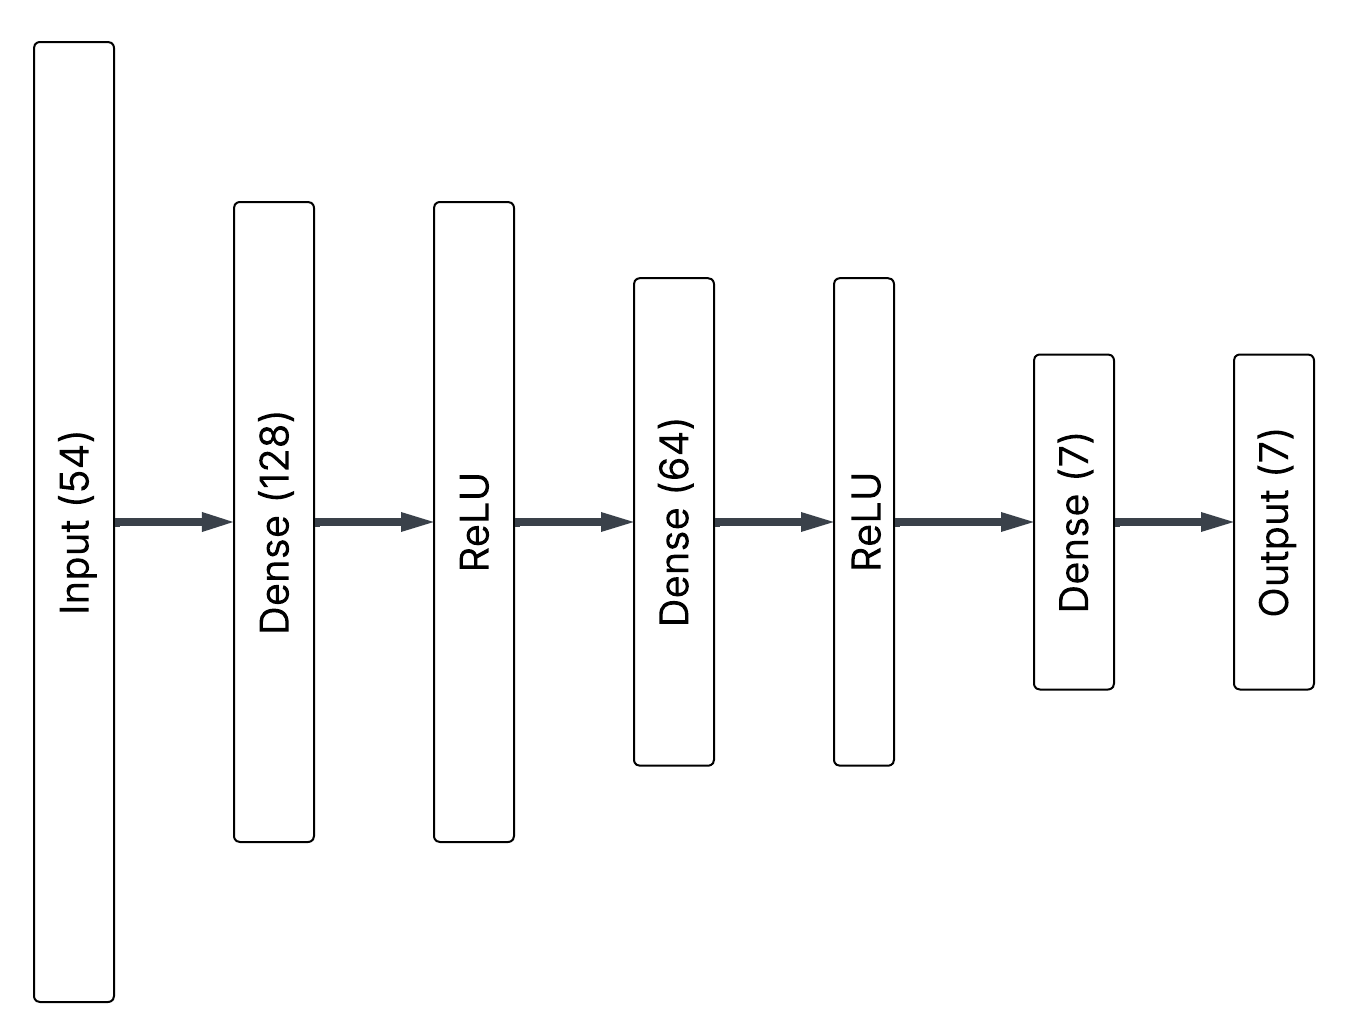
\includegraphics[height=0.28\textheight,width=0.6\textwidth]{Figures/Results/Covertype/Covertype_base_mlp_architecture.png} 
    \captionsetup{justification=centering}  % Ensure the caption is centered
    \caption{base\_mlp architecture for Covertype}
    \label{fig:covertypeMlpBaseArch}
\end{figure}

\begin{table}[h!]
    \centering
    \begin{tabular}{|l|l|l|l|l|l|l|}
    \hline
    \textbf{Model} & \textbf{param\_count} & \textbf{best\_acc} & \textbf{time\_best} & \textbf{train\_eff} & \textbf{auc\_eff} & \textbf{thru\_eff} \\
    \hline
    base\_mlp & 15,751 & 83.79\% & 64.17s & 0.013 & 121.207 & 1.920 \\
    fw\_spn & 20,481 & 85.41\% & 77.07s & 0.011 & 122.954 & 1.554 \\
    min\_spn & 12,289 & 82.19\% & 50.29s & 0.016 & 118.906 & 2.354 \\
    min\_mlp & 11,911 & \cellcolor{red!25}81.88\% & \cellcolor{green!25}48.05s & \cellcolor{green!25}0.017 & \cellcolor{red!25}118.777 & \cellcolor{green!25}2.505 \\
    max\_spn & 30,646 & 87.57\% & \cellcolor{red!25}2430.20s & \cellcolor{red!25}0.0003 & \cellcolor{green!25}127.573 & \cellcolor{red!25}0.042 \\
    pruned\_spn & 30,520 & \cellcolor{green!25}87.64\% & 2082.85s & 0.0004 & 127.413 & 0.055 \\
    \hline
    \end{tabular}
    \caption{Covertype Dataset results}
    \label{tab:covertypeResults}
\end{table}

\begin{enumerate}
\item \textbf{Baseline MLP vs. Free Weights SPN}: The fw\_spn model achieved the highest test accuracy, clearly outperforming the base\_mlp, which had the lowest accuracy out of all the models. The notable increase in parameter count of the fw\_spn, while retaining the same layer layout as the base\_mlp, correlates positively with its improved accuracy, providing strong evidence that enhanced internal connectivity boosts model performance. Although fw\_spn had slightly lower training and throughput efficiencies than the base\_mlp, this trade-off was justified by the considerable gain in accuracy.
\item \textbf{Minimal MLP vs. Minimal SPN}: Both min\_spn and min\_mlp achieved better accuracy compared to base\_mlp but slightly lower than fw\_spn. This suggests that having a higher param\_count might be more advantageous in this dataset than having more layers. Min\_spn consistently outperformed min\_mlp across all metrics except throughput efficiency, where both models were fairly close to one another. This further emphasizes the benefit of increased neural connectivity on model performance.
\item \textbf{Maximal SPN}: Max\_spn model had the third-highest accuracy but required significantly longer training times compared to the other models. This suggests a performance ceiling for the MNIST dataset, where additional internal connections yield diminishing returns.
\item \textbf{Pruned SPN}:
\begin{center}  % Centers the table
\begin{tabular}{|l|l|}
\hline
\textbf{Metric} & \textbf{Value} \\
\hline
Layers Before Pruning & 199 \\
Layers After Pruning & 105 \\
Mean Epoch Time Before Pruning & 20.39s \\
Mean Epoch Time After Pruning & 15.66s \\
Pruning Time & 293.63s \\
Pruning Effectiveness & 1.30 \\
\hline
\end{tabular}
\end{center}
The pruned\_spn model achieved accuracy similar to max\_spn while dramatically improving computational efficiency. Although the pruning process itself was time-consuming, taking longer than it took max\_spn to reach its peak accuracy (making it practically unusable), it still made the max\_spn model nearly 10x faster in average training time, validating the efficacy of pruning for optimizing maximal SPNs. Additionally, this pruning confirmed that a three-layer architecture is sufficient for optimal performance on this dataset. 

However, since max\_spn did not outperform any of the other models, it suggests that there was limited additional learning to be done, making pruning easier on this particular dataset.
\end{enumerate}

\begin{figure}[H]
    \centering
    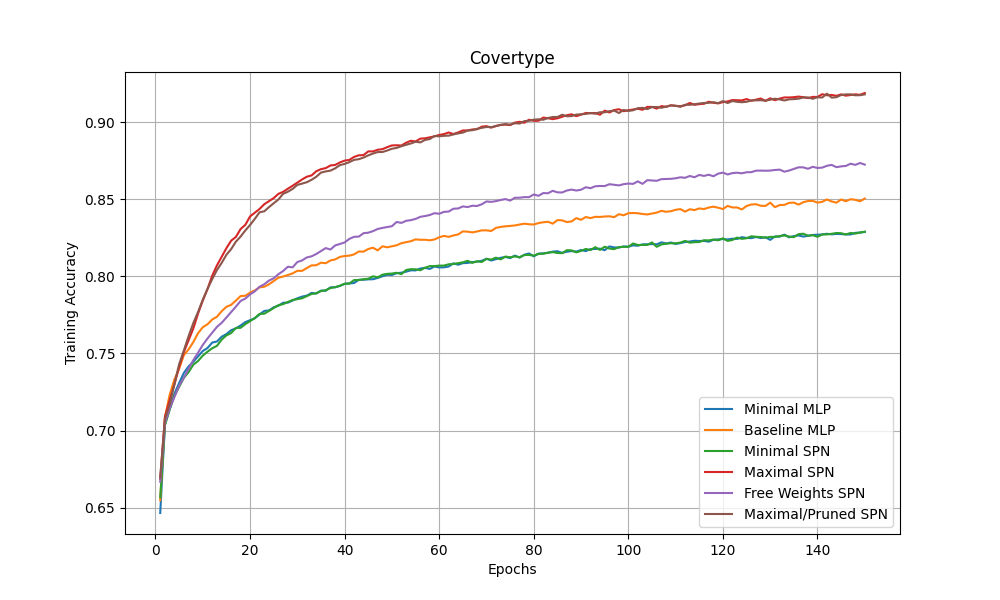
\includegraphics[width=\linewidth]{Figures/Results/Covertype/training_accuracy_plot.png} % first figure itself
    \captionsetup{width=\linewidth}
    \caption{train\_acc vs epochs curve for Covertype}
    \label{fig:covertypeTrainCurve}
\end{figure}

\begin{figure}[H]
    \centering
    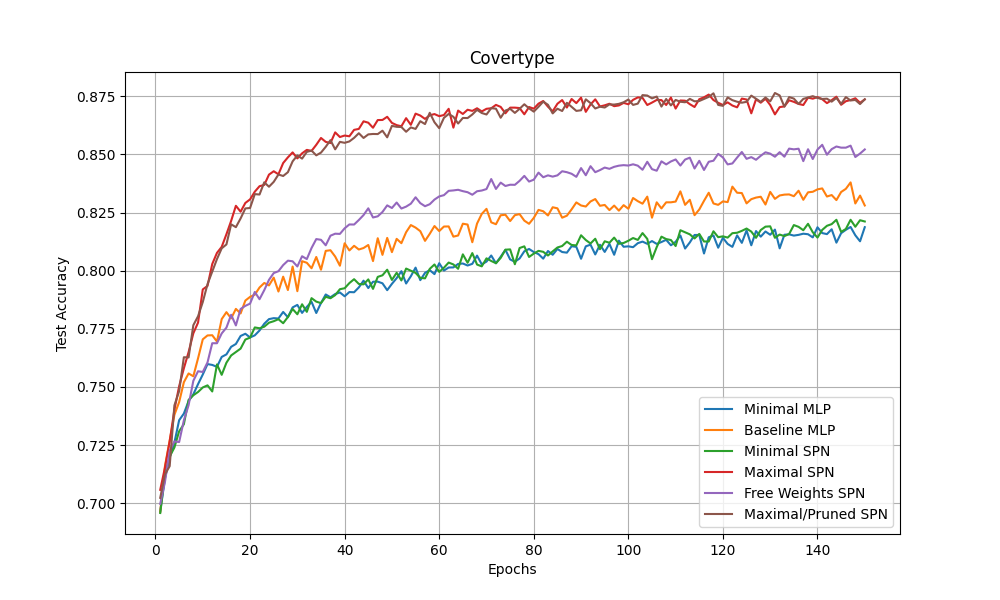
\includegraphics[width=\linewidth]{Figures/Results/Covertype/test_accuracy_plot.png} % second figure itself
    \captionsetup{width=\linewidth}
    \caption{test\_acc vs epochs curve for Covertype}
    \label{fig:covertyoeTestCurve}
\end{figure}

Overall, SPNs convincingly outperformed their MLP counterparts on the MNIST dataset. Maximal and pruned SPNs confirmed the existence of an upper performance bound, highlighting the effectiveness of strategic pruning to balance accuracy and efficiency.

\section{Language Domain Results}

\subsection{Newsgroups 20 Dataset}

\begin{tabular}{@{}ll@{}}
\textbf{Variant} & Simple \\
\textbf{Input Features} & 5000 \\
\textbf{Output Classes} & 20 \\
\textbf{Batch Size} & 64 \\
\textbf{Training Epochs} & 50 \\
\textbf{Training Samples} & 13,192 \\
\textbf{Test Samples} & 5,654 \\
\textbf{Base MLP Dimensions} & $[16,\, 8,\, 20]$ \\
\textbf{Total Neurons} & 44 \\
\end{tabular}

\begin{figure}[H]
    \centering
    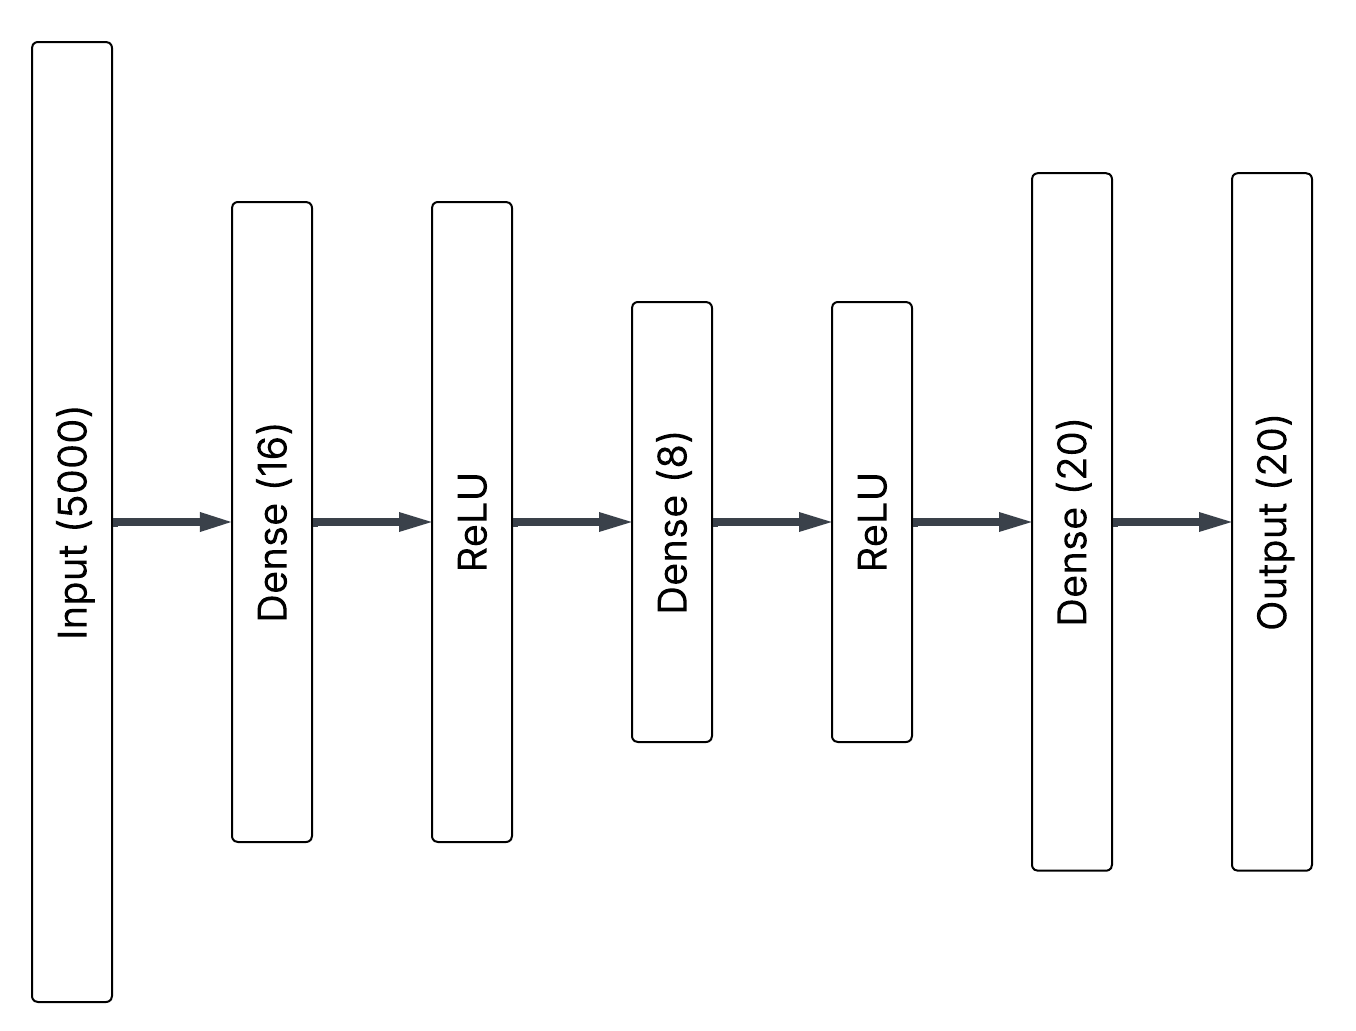
\includegraphics[height=0.28\textheight,width=0.6\textwidth]{Figures/Results/Newsgroups/Newsgroups_base_mlp_architecture.png} 
    \captionsetup{justification=centering}  % Ensure the caption is centered
    \caption{base\_mlp architecture for Newsgroups 20}
    \label{fig:newsgroupsMlpBaseArch}
\end{figure}

\begin{table}[h!]
    \centering
    \begin{tabular}{|l|l|l|l|l|l|l|}
    \hline
    \textbf{Model} & \textbf{param\_count} & \textbf{best\_acc} & \textbf{time\_best} & \textbf{train\_eff} & \textbf{auc\_eff} & \textbf{thru\_eff} \\
    \hline
    base\_mlp & 80,332 & \cellcolor{red!25}81.00\% & 0.77s & 1.054 & \cellcolor{red!25}38.869 & 2.938 \\
    fw\_spn & 220,652 & 87.48\% & \cellcolor{green!25}0.64s & \cellcolor{green!25}1.371 & 41.990 & 2.757 \\
    min\_spn & 220,524 & \cellcolor{green!25}88.82\% & 2.14s & 0.415 & \cellcolor{green!25}43.105 & \cellcolor{green!25}4.270 \\
    min\_mlp & 120,524 & 88.33\% & 0.91s & 0.967 & 42.720 & 3.937 \\
    max\_spn & 220,990 & 85.30\% & \cellcolor{red!25}7.99s & \cellcolor{red!25}0.107 & 41.103 & \cellcolor{red!25}0.217 \\
    pruned\_spn & 220,834 & 86.63\% & 1.39s & 0.625 & 41.356 & 1.265 \\
    \hline
    \end{tabular}
    \caption{Newsgroups 20 Dataset results}
    \label{tab:newsgroupsResults}
\end{table}

\begin{enumerate}
\item \textbf{Baseline MLP vs. Free Weights SPN}: The fw\_spn model achieved the highest test accuracy, clearly outperforming the base\_mlp, which had the lowest accuracy out of all the models. The notable increase in parameter count of the fw\_spn, while retaining the same layer layout as the base\_mlp, correlates positively with its improved accuracy, providing strong evidence that enhanced internal connectivity boosts model performance. Although fw\_spn had slightly lower training and throughput efficiencies than the base\_mlp, this trade-off was justified by the considerable gain in accuracy.
\item \textbf{Minimal MLP vs. Minimal SPN}: Both min\_spn and min\_mlp achieved better accuracy compared to base\_mlp but slightly lower than fw\_spn. This suggests that having a higher param\_count might be more advantageous in this dataset than having more layers. Min\_spn consistently outperformed min\_mlp across all metrics except throughput efficiency, where both models were fairly close to one another. This further emphasizes the benefit of increased neural connectivity on model performance.
\item \textbf{Maximal SPN}: Max\_spn model had the third-highest accuracy but required significantly longer training times compared to the other models. This suggests a performance ceiling for the MNIST dataset, where additional internal connections yield diminishing returns.
\item \textbf{Pruned SPN}:
\begin{center}  % Centers the table
\begin{tabular}{|l|l|}
\hline
\textbf{Metric} & \textbf{Value} \\
\hline
Layers Before Pruning & 24 \\
Layers After Pruning & 7 \\
Mean Epoch Time Before Pruning & 3.87s \\
Mean Epoch Time After Pruning & 0.69s \\
Pruning Time & 70.55s \\
Pruning Effectiveness & 5.61 \\
\hline
\end{tabular}
\end{center}
The pruned\_spn model achieved accuracy similar to max\_spn while dramatically improving computational efficiency. Although the pruning process itself was time-consuming, taking longer than it took max\_spn to reach its peak accuracy (making it practically unusable), it still made the max\_spn model nearly 10x faster in average training time, validating the efficacy of pruning for optimizing maximal SPNs. Additionally, this pruning confirmed that a three-layer architecture is sufficient for optimal performance on this dataset. 

However, since max\_spn did not outperform any of the other models, it suggests that there was limited additional learning to be done, making pruning easier on this particular dataset.
\end{enumerate}

\begin{figure}[H]
    \centering
    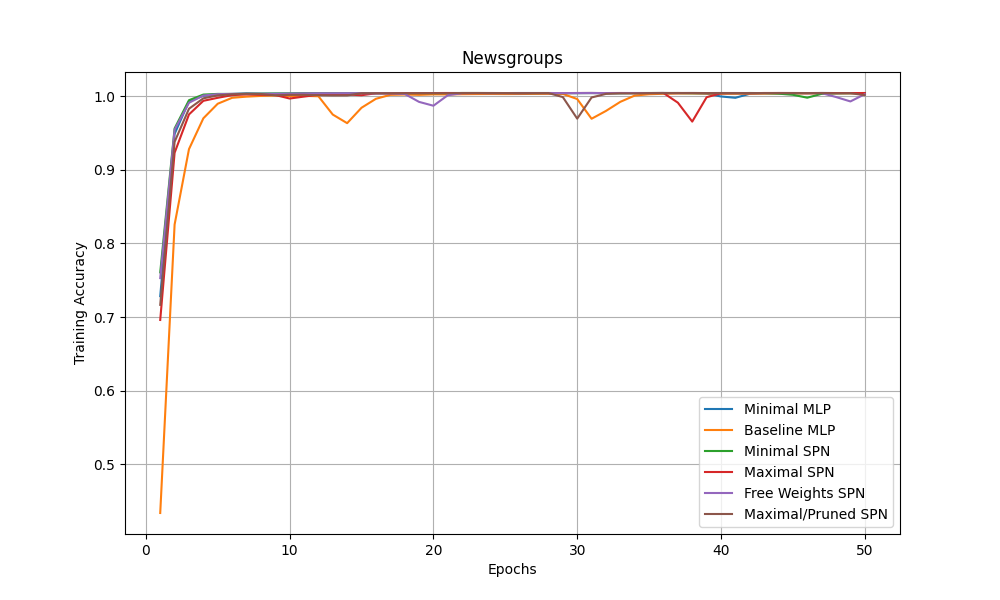
\includegraphics[width=\linewidth]{Figures/Results/Newsgroups/training_accuracy_plot.png} % first figure itself
    \captionsetup{width=\linewidth}
    \caption{train\_acc vs epochs curve for Newsgroups 20}
    \label{fig:newsgroupsTrainCurve}
\end{figure}

\begin{figure}[H]
    \centering
    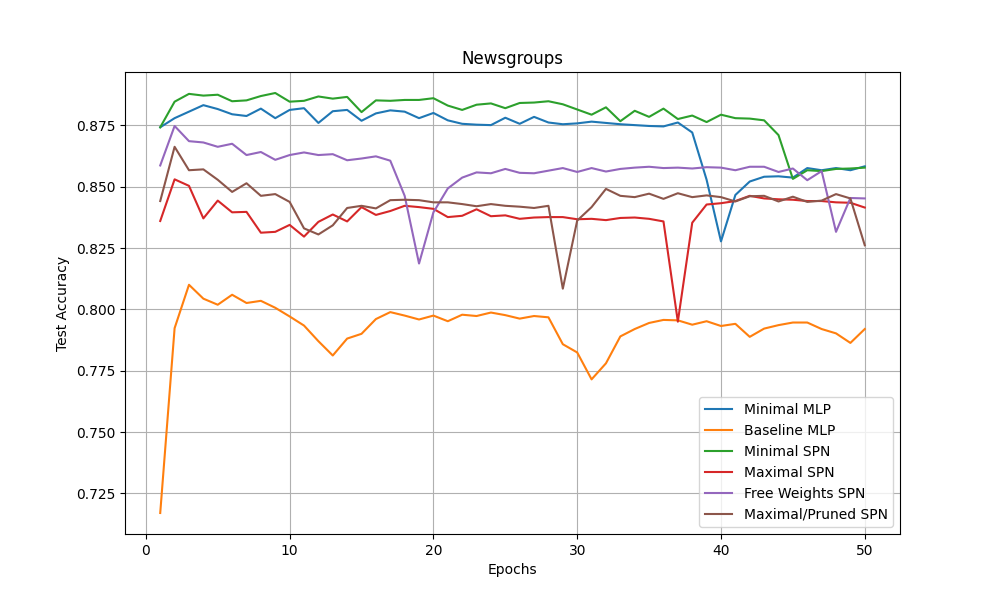
\includegraphics[width=\linewidth]{Figures/Results/Newsgroups/test_accuracy_plot.png} % second figure itself
    \captionsetup{width=\linewidth}
    \caption{test\_acc vs epochs curve for Newsgroups 20}
    \label{fig:newsgroupsTestCurve}
\end{figure}

Overall, SPNs convincingly outperformed their MLP counterparts on the MNIST dataset. Maximal and pruned SPNs confirmed the existence of an upper performance bound, highlighting the effectiveness of strategic pruning to balance accuracy and efficiency.

\subsection{IMDB Reviews Dataset}

\begin{tabular}{@{}ll@{}}
\textbf{Variant} & Complex \\
\textbf{Input Features} & 5000 \\
\textbf{Output Classes} & 2 \\
\textbf{Batch Size} & 32 \\
\textbf{Training Epochs} & 50 \\
\textbf{Training Samples} & 25,000 \\
\textbf{Test Samples} & 25,000 \\
\textbf{Base MLP Dimensions} & $[64,\, 32,\, 2]$ \\
\textbf{Total Neurons} & 96 \\
\end{tabular}

\begin{figure}[H]
    \centering
    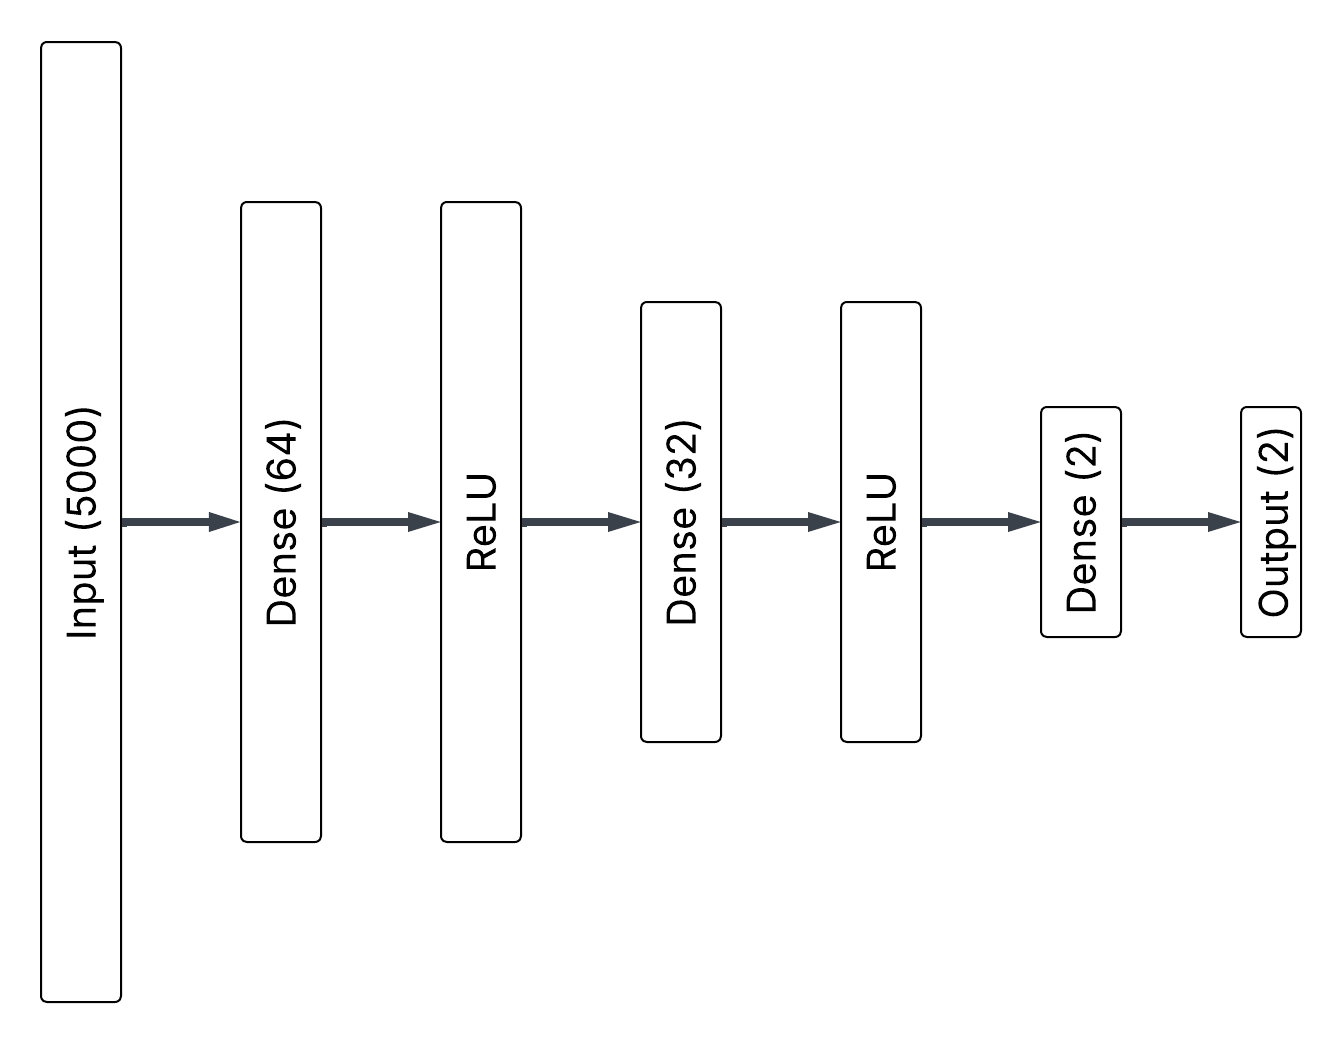
\includegraphics[height=0.28\textheight,width=0.6\textwidth]{Figures/Results/IMDB/IMDB_base_mlp_architecture.png} 
    \captionsetup{justification=centering}  % Ensure the caption is centered
    \caption{base\_mlp architecture for IMDB Reviews}
    \label{fig:imdbMlpBaseArch}
\end{figure}

\begin{table}[h!]
    \centering
    \begin{tabular}{|l|l|l|l|l|l|l|}
    \hline
    \textbf{Model} & \textbf{param\_count} & \textbf{best\_acc} & \textbf{time\_best} & \textbf{train\_eff} & \textbf{auc\_eff} & \textbf{thru\_eff} \\
    \hline
    base\_mlp & 322,210 & 86.70\% & 1.09s & 0.792 & \cellcolor{red!25}41.175 & 0.787 \\
    fw\_spn & 492,338 & \cellcolor{green!25}86.87\% & 1.53s & 0.569 & 41.360 & 0.550 \\
    min\_spn & 490,290 & \cellcolor{red!25}86.34\% & \cellcolor{green!25}0.90s & \cellcolor{green!25}0.955 & \cellcolor{green!25}41.455 & 0.954 \\
    min\_mlp & 480,290 & 85.99\% & 1.85s & 0.466 & 41.319 & \cellcolor{green!25}1.009 \\
    max\_spn & 494,851 & 86.84\% & \cellcolor{red!25}35.29s & \cellcolor{red!25}0.025 & 41.340 & \cellcolor{red!25}0.025 \\
    pruned\_spn & 494,810 & 86.64\% & 27.01s & 0.032 & 41.255 & 0.032 \\
    \hline
    \end{tabular}
    \caption{IMDB Reviews Dataset results}
    \label{tab:imdbResults}
\end{table}

\begin{enumerate}
\item \textbf{Baseline MLP vs. Free Weights SPN}: The fw\_spn model achieved the highest test accuracy, clearly outperforming the base\_mlp, which had the lowest accuracy out of all the models. The notable increase in parameter count of the fw\_spn, while retaining the same layer layout as the base\_mlp, correlates positively with its improved accuracy, providing strong evidence that enhanced internal connectivity boosts model performance. Although fw\_spn had slightly lower training and throughput efficiencies than the base\_mlp, this trade-off was justified by the considerable gain in accuracy.
\item \textbf{Minimal MLP vs. Minimal SPN}: Both min\_spn and min\_mlp achieved better accuracy compared to base\_mlp but slightly lower than fw\_spn. This suggests that having a higher param\_count might be more advantageous in this dataset than having more layers. Min\_spn consistently outperformed min\_mlp across all metrics except throughput efficiency, where both models were fairly close to one another. This further emphasizes the benefit of increased neural connectivity on model performance.
\item \textbf{Maximal SPN}: Max\_spn model had the third-highest accuracy but required significantly longer training times compared to the other models. This suggests a performance ceiling for the MNIST dataset, where additional internal connections yield diminishing returns.
\item \textbf{Pruned SPN}:
\begin{center}  % Centers the table
\begin{tabular}{|l|l|}
\hline
\textbf{Metric} & \textbf{Value} \\
\hline
Layers Before Pruning & 96 \\
Layers After Pruning & 63 \\
Mean Epoch Time Before Pruning & 35.20s \\
Mean Epoch Time After Pruning & 27.01s \\
Pruning Time & 253.58s \\
Pruning Effectiveness & 1.30 \\
\hline
\end{tabular}
\end{center}
The pruned\_spn model achieved accuracy similar to max\_spn while dramatically improving computational efficiency. Although the pruning process itself was time-consuming, taking longer than it took max\_spn to reach its peak accuracy (making it practically unusable), it still made the max\_spn model nearly 10x faster in average training time, validating the efficacy of pruning for optimizing maximal SPNs. Additionally, this pruning confirmed that a three-layer architecture is sufficient for optimal performance on this dataset. 

However, since max\_spn did not outperform any of the other models, it suggests that there was limited additional learning to be done, making pruning easier on this particular dataset.
\end{enumerate}

\begin{figure}[H]
    \centering
    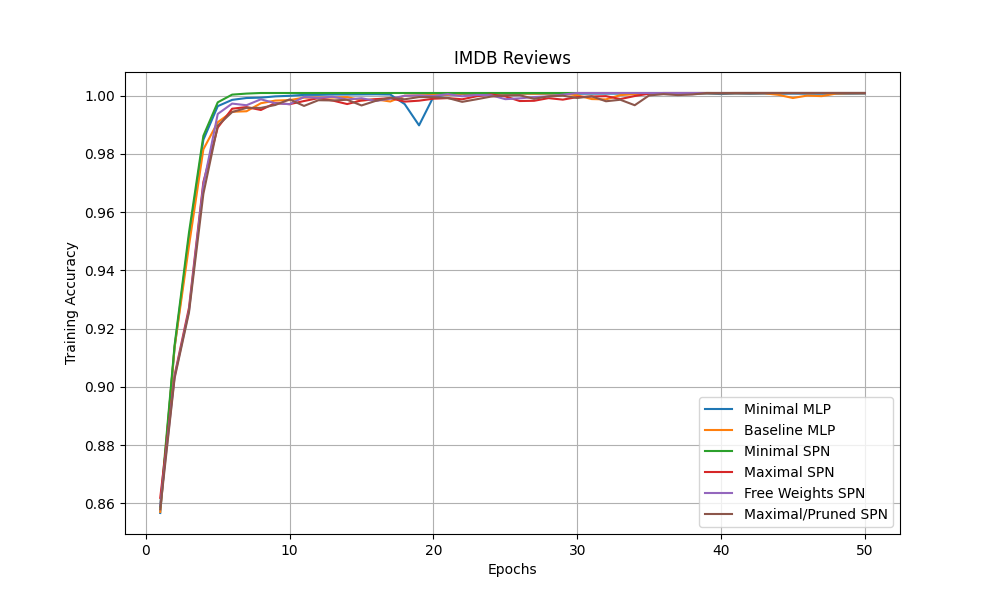
\includegraphics[width=\linewidth]{Figures/Results/IMDB/training_accuracy_plot.png} % first figure itself
    \captionsetup{width=\linewidth}
    \caption{train\_acc vs epochs curve for IMDB Reviews}
    \label{fig:imdbTrainCurve}
\end{figure}

\begin{figure}[H]
    \centering
    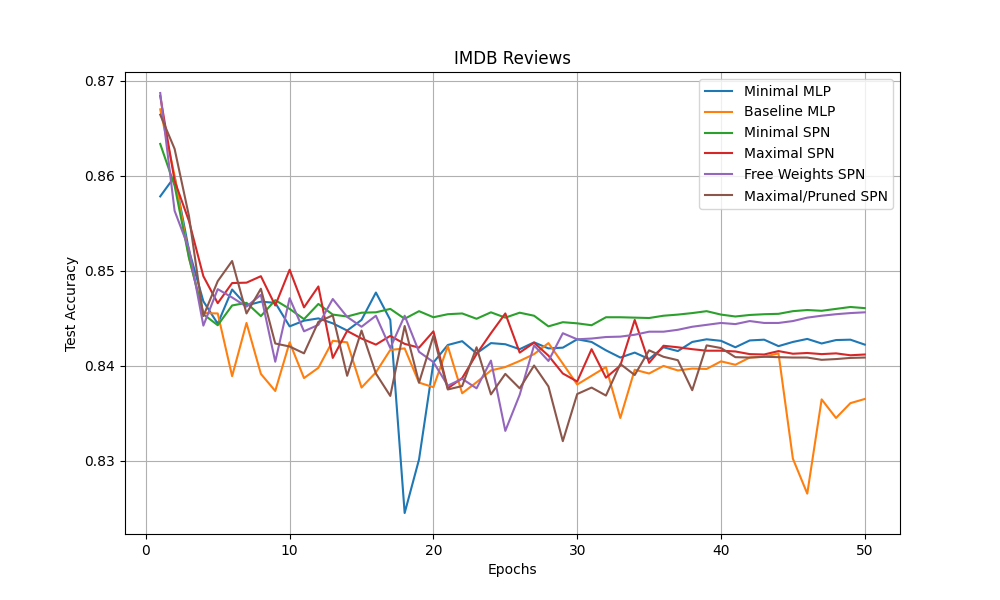
\includegraphics[width=\linewidth]{Figures/Results/IMDB/test_accuracy_plot.png} % second figure itself
    \captionsetup{width=\linewidth}
    \caption{test\_acc vs epochs curve for IMDB Reviews}
    \label{fig:imdbTestCurve}
\end{figure}

Overall, SPNs convincingly outperformed their MLP counterparts on the MNIST dataset. Maximal and pruned SPNs confirmed the existence of an upper performance bound, highlighting the effectiveness of strategic pruning to balance accuracy and efficiency.

%-----------------------------------
%	SUBSECTION 1
%-----------------------------------
\subsection{Subsection 1}

Nunc posuere quam at lectus tristique eu ultrices augue venenatis. Vestibulum ante ipsum primis in faucibus orci luctus et ultrices posuere cubilia Curae; Aliquam erat volutpat. Vivamus sodales tortor eget quam adipiscing in vulputate ante ullamcorper. Sed eros ante, lacinia et sollicitudin et, aliquam sit amet augue. In hac habitasse platea dictumst.

%-----------------------------------
%	SUBSECTION 2
%-----------------------------------

\subsection{Subsection 2}
Morbi rutrum odio eget arcu adipiscing sodales. Aenean et purus a est pulvinar pellentesque. Cras in elit neque, quis varius elit. Phasellus fringilla, nibh eu tempus venenatis, dolor elit posuere quam, quis adipiscing urna leo nec orci. Sed nec nulla auctor odio aliquet consequat. Ut nec nulla in ante ullamcorper aliquam at sed dolor. Phasellus fermentum magna in augue gravida cursus. Cras sed pretium lorem. Pellentesque eget ornare odio. Proin accumsan, massa viverra cursus pharetra, ipsum nisi lobortis velit, a malesuada dolor lorem eu neque.

%----------------------------------------------------------------------------------------
%	SECTION 2
%----------------------------------------------------------------------------------------

\section{Main Section 2}

Sed ullamcorper quam eu nisl interdum at interdum enim egestas. Aliquam placerat justo sed lectus lobortis ut porta nisl porttitor. Vestibulum mi dolor, lacinia molestie gravida at, tempus vitae ligula. Donec eget quam sapien, in viverra eros. Donec pellentesque justo a massa fringilla non vestibulum metus vestibulum. Vestibulum in orci quis felis tempor lacinia. Vivamus ornare ultrices facilisis. Ut hendrerit volutpat vulputate. Morbi condimentum venenatis augue, id porta ipsum vulputate in. Curabitur luctus tempus justo. Vestibulum risus lectus, adipiscing nec condimentum quis, condimentum nec nisl. Aliquam dictum sagittis velit sed iaculis. Morbi tristique augue sit amet nulla pulvinar id facilisis ligula mollis. Nam elit libero, tincidunt ut aliquam at, molestie in quam. Aenean rhoncus vehicula hendrerit.